\chapter{Methods}

\section{System of Equations}
The system of study was modelled using coupled Ordinary Differential Equations (ODEs). The model is based on a logistic framework modified with a dynamic carrying capacity that depends on the environmental conditions. The ``environment" consists of the resources, oxygen and testosterone which have their own equations for production and consumption. We make the simplifying assumption that every other resource required by cells are present in non-limiting concentrations. Additionally, the cell types were assumed to not mutate and hence cannot change their types. No spatial structure is considered and the system is assumed to be well mixed and the resource available in bulk for all the cells.

The ODEs for population size of a cell type is given in \autoref{cell_eq}. The equation is such that the population increases by a maximum growth rate $r_{i,max}$ and reduces by a maximum death rate $\delta_i$. The effective growth rate decreases as the total population approaches a maximum limit while the effective death rate stays the same. This maximum limit for the total population varies between 1 to $K_{i,max}$ and varies depending on the resource availability as a function of the form as given in \autoref{fres_eq} and visualised in \autoref{fig_fres}.\\
For $i \in \{T^+,T^p,T^-\}$
\begin{equation}
  \frac{dy_i}{dt} = r_{i,max}(dtx) y_i (1 - \frac{\sum_j y_j}{1 + K_{i,max} f_i(O_2) f_i(test)} )- \delta_i y_i
  \label{cell_eq}
\end{equation}

The functional dependence on resource $f_i(res) \in [0,1]$. Below the lower limit, $ll_{res,i}$ the function is 0, representative of no growth, and increases linearly above it upto the upper limit, $ul_{res,i}$ and the function saturates to 1, representative of the maximum growth, for any resource levels above that.\\
For $res \in \{O_2,test\}$
\begin{equation}
  f_i(res) = \begin{cases}
  1 &\text{if } ul_{res,i} \leq res \\
  \frac{res-ll_{res,i}}{ul_{res,i}-ll_{res,i}} &\text{if } ll_{res,i} < res < ul_{res,i} \\
  0 &\text{if } res \leq ll_{res,i} \\
  \end{cases}
  \label{fres_eq}
\end{equation}
\begin{figure}[h]
  \centering
  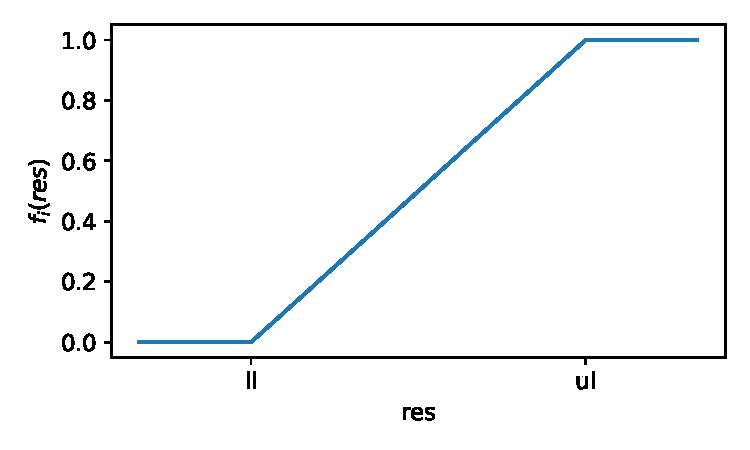
\includegraphics[width=0.5\textwidth]{f_res}
  \caption{$f_i(res)$}
  \label{fig_fres}
\end{figure}

The ODE for oxygen is given in \autoref{o2_eq}. This involves a term for external production that increase oxygen levels constantly at a rate $p_{O_2}$, a term for uptake by all cells where they decrease oxygen levels at a rate $\mu_{O_2,i}$ and a term for decay where oxygen level decreases at a rate $\lambda_{O_2}$.
\begin{equation}
  \frac{dO_2}{dt} = p_{O_2} - \sum_i \mu_{O_2,i} y_i - \lambda_{O_2} O_2
  \label{o2_eq}
\end{equation}

The ODE for testosterone is given in \autoref{test_eq}. The form is similar to that of oxygen, with the difference being production being done by $T^p$ cells at a rate $p_{test}$ here.
\begin{equation}
  \frac{dtest}{dt} = p_{test}(abi) y_{T^p} - \sum_i \mu_{test,i} y_i - \lambda_{test} test
  \label{test_eq}
\end{equation}

Note that these equations are defined only for positive values of cell count and resource level to be biologically relevant. To mitigate the problem of having a continuous variable for  cell count, $y_i < 1$ is defined as extinction of the cell type $i$ and $y_i = \frac{dy_i}{dt} = 0$ in such a case.

\section{Therapy}
For implementation of therapy, production rate of testosterone and growth rate of the cells are governed by the dose of abiraterone $abi$ and docetaxel $dtx$ respectively as given in \autoref{p_test_dose_eq} and \autoref{r_dose_eq}. Therapy is modelled as a boolean value, where $1$ represents dose at MTD and $0$ represents no dose.
\begin{equation}
  p_{test}(abi) = \begin{cases}
  p_{test,max} &\text{if } abi = 0 \\
  p_{test,min} &\text{if } abi = 1 \\
  \end{cases}
  \label{p_test_dose_eq}
\end{equation}
\begin{equation}
  r_i(dtx) = \begin{cases}
  r_{i,max} &\text{if } dtx = 0 \\
  r_{i,min} &\text{if } dtx = 1 \\
  \end{cases}
  \label{r_dose_eq}
\end{equation}
The dosing scheme for standard-of-care is given in \autoref{dose_soc_eq}. Here, the dose is applied at MTD at all times from the start of the simulation regardless of the population size.\\
For $dose \in \{abi,dtx\}$
\begin{equation}
  dose(x,t) = 1 \quad \forall\ t, x
  \label{dose_soc_eq}
\end{equation}

The dosing scheme for adaptive therapy is given in \autoref{dose_at_eq}. A binary mode of adaptive therapy is considered here, where dose is applied at MTD when the population size exceeds the $on$ threshold and stays on until the population size falls below the $off$ threshold, after which it is turned off.
\begin{equation}
  dose(x,t) = \begin{cases}
  0 &\text{if } dose(x,t-\Delta t) = 0 \text{ and } x < on\\
  1 &\text{if } dose(x,t-\Delta t) = 0 \text{ and } x \geq on \\
  1 &\text{if } dose(x,t-\Delta t) = 1 \text{ and } x > off \\
  0 &\text{if } dose(x,t-\Delta t) = 1 \text{ and } x \leq off \\
  \end{cases}
  \label{dose_at_eq}
\end{equation}

\section{Constraint equations and parameters from literature}
\autoref{parmtable} gives a brief description of the parameters from the above equations, the values used, and the sources for these values where applicable. Note that all the resource parameters are normalised to ``Tissue levels of that resource" as obtained from the literature sources cited. The cell lines of LNCaP, 22Rv1 and PC3 were considered to correspond to the $T^+$, $T^p$ and $T^-$ cells respectively when obtaining literature values.

Constraint equations given below were used to determine the values of some parameters for which direct sources were not available.\\
\autoref{r_eq} is obtained from solving \autoref{cell_eq} from $N_0$ to $2N_0$ under the assumption that resources are not limiting and $y_i$ is small. This constraint along with doubling time and death rates obtained from literature can be used to get the growth rate.
\begin{equation}
  r_{i,max} = \frac{ln(2)}{\tau_{d,i}} + \delta_i
  \label{r_eq}
\end{equation}
\autoref{K_eq} is obtained from setting \autoref{cell_eq} = 0 under the assumption that equilibrium is reached with only one cell type present and resources are not limited. This constraint along with an assumed equilibrium value of 10000 for the cells, growth and death rate obtained from above can be used to get the maximum carrying capacity for that cell type.
\begin{equation}
  K_{i,max}=\frac{r_{i,max}}{r_{i,max}-\delta_i} y_i^*
  \label{K_eq}
\end{equation}
\autoref{p_o2_eq} is obtained from setting \autoref{o2_eq} = 0 under the assumption that equilibrium is reached with only $T^-$ cell type present. This constraint along with an assumed equilibrium value of 1 for oxygen and 10000 for the cells, and uptake and decay rates from literature can be used to get the production rate of oxygen.
\begin{equation}
  p_{O_2} = \lambda_{O_2} O_2^* + y_i^* \mu_i
  \label{p_o2_eq}
\end{equation}
\autoref{p_test_eq} is obtained from setting \autoref{test_eq} = 0 under the assumption that equilibrium is reached with only $T^p$ cell type present. This constraint along with an assumed equilibrium value of 1 for oxygen and 10000 for the cells, decay rates from literature can be used to get the production rate of testosterone.
\begin{equation}
  p_{test,max} - \mu_{test,T^p} = \frac{test^* \lambda_{test}}{y_{T^p}^*} = 4 \times 10^{-4}
  \label{p_test_eq}
\end{equation}
\autoref{p_test_doseparm_eq} is the same as \autoref{p_test_eq} with a lower equilibrium value of testosterone with abiraterone therapy.
\begin{equation}
  p_{test,min} = \frac{test_{abi}^* \lambda_{test}}{y_{T^p}^*} + \mu_{test,T^p}
  \label{p_test_doseparm_eq}
\end{equation}
\autoref{r_doseparm_eq} is the rearranged version of \autoref{K_eq} with a lower equilibrium value for the cells with docetaxel therapy.
\begin{equation}
  r_{i,min}=\frac{K_{i,max}}{K_{i,max} - y_{i,dtx}^*} \delta_i
  \label{r_doseparm_eq}
\end{equation}

\section{Code Implementation}
The code is written in Python 3 and with dependencies of numpy, scipy, pandas, matplotlib and seaborn libraries. The system of equations were solved numerically by the LSODA algorithm provided by the \texttt{scipy.integrate.ode} function. The code is designed to iterate over the different parameters of a set parallely over multiple threads, however, the actual solver is sequential and single threaded.

The code, at each time step checks if the values are non-negative and sets them to 0 if it is the case. This is since the equations are not defined in these range of values and numerical errors can give rise to negative values. A similar implementation is done for $y_i < 1$.

The source code along with the data is available at the following Github repository: \url{https://www.github.com/harshavardhan-bv/cancer-compe-strat}.
\begin{figure}[h]
  \centering
  
\includegraphics[width=0.15\textwidth]{github}
  \caption{QR code for the Github repository}
  \label{github}
\end{figure}


\newpage
\begin{longtable}[c]{|l|p{4.3cm}|c|p{2.3cm}|}

  \hline \multicolumn{1}{|c|}{\textbf{Parameter}} & \multicolumn{1}{c|}{\textbf{Description}} & \multicolumn{1}{c|}{\textbf{Value(s)}} & \multicolumn{1}{c|}{\textbf{Source(s)}}\\ \hline
  \endhead

  \hline \multicolumn{4}{|r|}{{Continued on next page}} \\ \hline
  \endfoot

  \endlastfoot

  $y_i$ & No. of cells of cell type $i$ & N/A & N/A  \\ \hline
  $r_{i,max}$ & Population growth rate of cell type $i$  &
  \begin{tabular}{l|l}
    $T^+$ & $2.84 \times 10^{-3}$ \tiny{min$^{-1}$}\\
    $T^p$ & $2.79 \times 10^{-3}$ \tiny{min$^{-1}$}\\
    $T^-$ & $6.23 \times 10^{-4}$ \tiny{min$^{-1}$}\\
  \end{tabular}
  & \autoref{r_eq} \\ \hline
  $r_{i,min}$ & Population growth rate of cell type $i$ under $dtx$ therapy &
  \begin{tabular}{l|l}
    $T^+$ & $2.55 \times 10^{-3}$ \tiny{min$^{-1}$}\\
    $T^p$ & $2.54 \times 10^{-3}$ \tiny{min$^{-1}$}\\
    $T^-$ & $2.06 \times 10^{-4}$ \tiny{min$^{-1}$}\\
  \end{tabular}
  & \autoref{r_doseparm_eq} \\ \hline
  $\delta_i$  & Population death rate of cell type $i$ &
  \begin{tabular}{l|l}
    $T^+$ & $2.5 \times 10^{-3}$ \tiny{min$^{-1}$}\\
    $T^p$ & $2.5 \times 10^{-3}$ \tiny{min$^{-1}$}\\
    $T^-$ & $1.6 \times 10^{-4}$ \tiny{min$^{-1}$}\\
  \end{tabular}
  & \cite{Jain}  \\ \hline
  $K_{i,max}$ & Maximum Carrying capacity, coming up through the environment/resources &
  \begin{tabular}{l|l}
    $T^+$ & $8.35 \times 10^4$ \\
    $T^p$ & $9.62 \times 10^4$ \\
    $T^-$ & $1.34 \times 10^4$ \\
  \end{tabular}
  & \autoref{K_eq} \\ \hline
  $f_{i,res}$ & Functional dependence of cell type $i$ on resource $res$, normalised to 1 & $f_{T^-,test}=1$ & N/A \\ \hline
  $p_{res}$ & Production rate of resource, either as bulk or by cells &
  \begin{tabular}{l|l}
    $O_2$ & 0.11 \tiny{min$^{-1}$}\\
    $test,max$ & $5 \times 10^{-7}$ \tiny{min$^{-1}$cell$^{-1}$}\\
  \end{tabular}
  & \autoref{p_o2_eq}, \autoref{p_test_eq}\\ \hline
  $p_{test,min}$ & Production rate of $test$ under $abi$ therapy & $1 \times 10^{-7}$ \tiny{min$^{-1}$cell$^{-1}$} & \autoref{p_test_doseparm_eq}\\ \hline
  $\mu_{res,i}$ & Uptake of resource $res$ by cell type $i$ &
  \begin{tabular}{l|l|l}
    $O_2$ & $T^+$ & $1.63 \times 10^{-6}$ \tiny{min$^{-1}$cell$^{-1}$}\\
    & $T^p$ & $1.63 \times 10^{-6}$ \tiny{min$^{-1}$cell$^{-1}$}\\
    & $T^-$ & $1.04 \times 10^{-6}$ \tiny{min$^{-1}$cell$^{-1}$}\\ \hline
    $test$ & $T^+$ & $2.34 \times 10^{-8}$ \tiny{min$^{-1}$cell$^{-1}$}\\
    & $T^p$ & $6.00 \times 10^{-8}$ \tiny{min$^{-1}$cell$^{-1}$}\\
    & $T^-$ & 0 \tiny{min$^{-1}$cell$^{-1}$}\\
  \end{tabular}
  & \cite{HailJr}, \autoref{p_test_eq}\\ \hline
  $\lambda_{res}$ & Decay rate of resource $res$ &
  \begin{tabular}{l|l}
    $O_2$ & 0.100 \tiny{min$^{-1}$}\\
    $test$ & 0.004 \tiny{min$^{-1}$}\\
  \end{tabular}
  & \cite{Jain}\\ \hline
  $ll_{res,i}$ & Lower limit/threshold level of resource $res$ for carrying capacity of cell type $i$ & $\in [0,1]$ & N/A \\ \hline
  $ul_{res,i}$ & Upper limit/saturation level of resource $res$ for carrying capacity of cell type $i$ & $\in [0,1]$ & N/A \\ \hline
  \multicolumn{4}{|c|}{Supplementary Parameters}\\ \hline
  $\tau_d$  & Doubling time of cell type $i$ &
  \begin{tabular}{l|l}
    $T^+$ & $34$ \tiny{hr} \\
    $T^p$ & $40$ \tiny{hr} \\
    $T^-$ & $25$ \tiny{hr} \\
  \end{tabular}
  & \cite{atcc} \\ \hline
  $y_i^*$ & Equilibrium value of cell number in absence of competition & 10000 & assumed \\ \hline
  $y_{i,dtx}^*$ & Equilibrium value of cell number in absence of competition under $dtx$ therapy &
  \begin{tabular}{l|l}
    $T^+$ & $0.30 \times y_i^*$ \\
    $T^p$ & $0.30 \times y_i^*$ \\
    $T^-$ & $0.15 \times y_i^*$ \\
  \end{tabular}
  & \cite{Morikawa} \\ \hline
  $res^*$ & Equilibrium/Tissue levels of resource with one cell type present &
  \begin{tabular}{l|l}
    $O_2$    & 2.5 \tiny{mmHg}          \\
    $test$   & 3.74 \tiny{pmol/g tissue}\\
  \end{tabular}
  & \cite{Steward},\cite{Titus} \\ \hline
  $test_{abi}^*$ & Equilibrium/Tissue levels of testosterone with only $T^p$ cell type present under $abi$ therapy & $0.1 \times test^*$ & \cite{Acharya} \\ \hline

  \caption{Table of all parameters}
  \label{parmtable}\\
\end{longtable}
